\paragraph{Tijdsduur}
\begin{figure}[H]
    \centering
    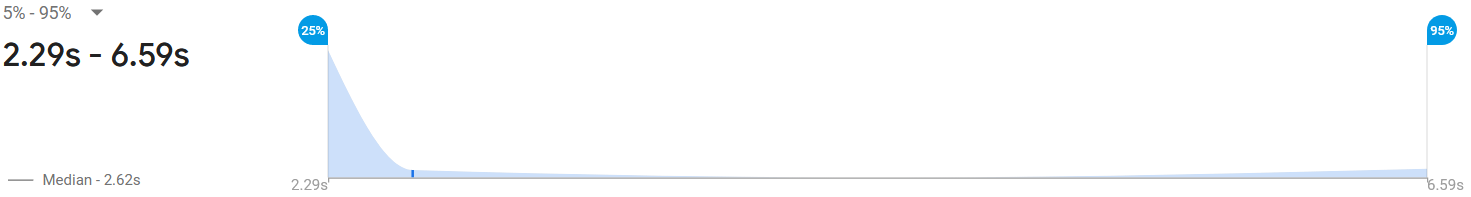
\includegraphics[height=0.1\textheight]{basisDuratieCross.png}
    \caption{Overzicht tijdsduur opstarten van applicatie met basisfunctionaliteiten bij React Native.}
\end{figure}
Tijdens het meten van de duur voor het opstarten van de applicatie, 
is de applicatie meerdere keren opgestart. Op de grafiek is te zien dat de applicatie
gemiddeld 2,84 seconden nodig heeft om op te starten. Het minimum en maximum
liggen op 2,29 en 6,59 seconden.

\paragraph{CPU \& geheugen}
\begin{figure}[H]
    \centering
    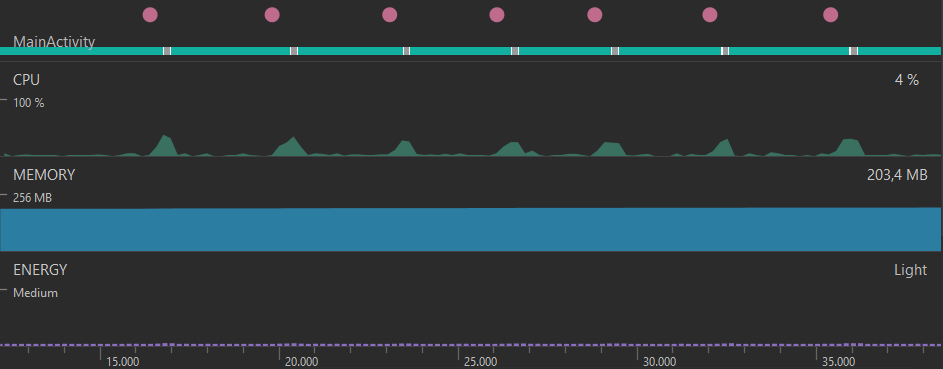
\includegraphics[height=0.25\textheight]{basisPerformantieCross.png}
    \caption{Overzicht CPU en geheugen gebruik tijdens het navigeren tussen schermen bij React Native.}
\end{figure}
Net zoals bij native is op de grafiek te zien dat het CPU gebruik van de applicatie wanneer deze
inactief is, rond de 4\% ligt. En dat er duidelijk zichtbaar is wanneer er
genavigeerd wordt tussen de schermen. De piek van het CPU gebruik lag gemiddeld
op 32\% met een minimum en maximum van 27\% en 40\%. Wat bij React Native opvalt is dat
het eerste keer navigeren naar een scherm een grotere piek geeft. Eenmaal dat het scherm 
al werd ingeladen is de piek minder groot. Dit wijst erop dat React Native gebruik maakt van
lazy loading. Het geheugen blijft in tegenstelling
met de CPU wanneer de applicatie inactief en actief is, rond de 202MB hangen, met
verschillen van maximum 4-5MB. Er is geen merkbaar verschil in het geheugen wanneer
er genavigeerd wordt tussen de schermen.
